\chapter{Courant Continu} \label{subsec:dc_circuit_theory}
La th\'eorie des circuits en courant continu (DC) pose les bases de l’\'electronique en
d\'ecrivant le comportement des tensions et courants statiques (invariants dans le temps)
dans des boucles ferm\'ees.\\

\begin{figure}[!h]
  \centering
  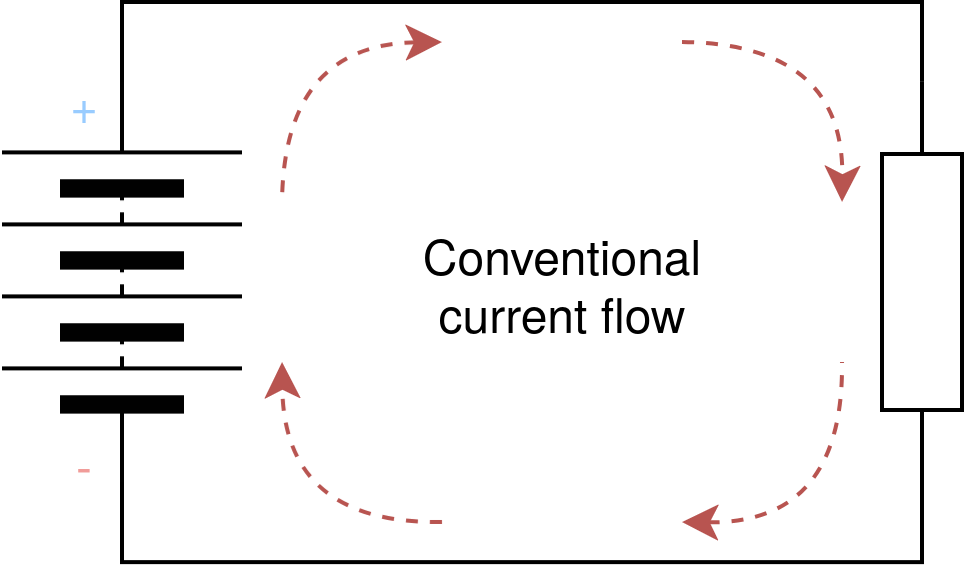
\includegraphics[width=0.6\textwidth]{current-flow.png}
  \caption{Le flux conventionnel du courant, de \(+\) vers --}
\end{figure}

\section{Les unit\'es trait\'ees} \label{subsec:units}
Avant d’aborder les circuits et les composants, il est important de d\'efinir
les \textit{unit\'es fondamentales} qui constituent le langage de l’\'electronique.
À la base se trouve la \textbf{charge \'electrique}, la grandeur fondamentale
qui sous-tend toutes les interactions \'electriques. De la charge d\'ecoule le \textbf{courant
\'electrique}, le flux de charges à travers un conducteur, et la \textbf{tension},
la diff\'erence de potentiel qui provoque ce flux. Les mat\'eriaux s’opposent au
mouvement des charges via leur \textbf{r\'esistance}, tandis que les notions
d’\textbf{\'energie} et de \textbf{puissance} permettent de d\'ecrire comment les circuits
stockent et d\'elivrent un travail utile. Ensemble, ces unit\'es \'etablissent le
cadre à travers lequel nous mesurons et analysons les ph\'enom\`enes \'electriques.\par
\vspace{\baselineskip}
\subsection{Charge \'electrique}\label{subsec:electric_charge}
La charge \'electrique est une propri\'et\'e fondamentale de la mati\`ere ; elle permet
les interactions via les champs \'electromagn\'etiques. Elle se quantifie en \textbf{coulombs
(\unit{\coulomb})}. Il existe deux types de charges \'electriques, qualifi\'ees de
positive et n\'egative. Les charges de m\^eme signe se repoussent, tandis que les charges
de signes oppos\'es s’attirent. Dans la mati\`ere ordinaire, le total des charges
positives et n\'egatives est \'equilibr\'e, une condition appel\'ee neutralit\'e \'electrique.
Les \'electrons (--) et les protons (\(+\)) sont les principaux porteurs de charge \'electrique.

\begin{figure}[H]
  \centering
  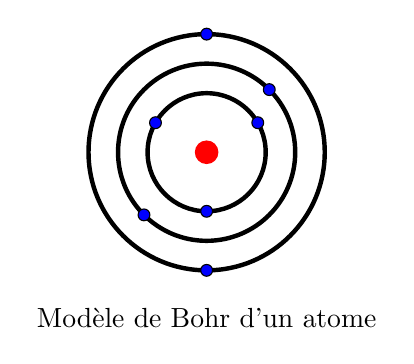
\begin{tikzpicture}[scale=0.75]
    \fill[red] (0,0) circle (0.2);
    \draw[ultra thick] (0,0) circle (1);
    \draw[ultra thick] (0,0) circle (1.5);
    \draw[ultra thick] (0,0) circle (2);
    \foreach \theta in {30, 150, 270}
    \draw[fill=blue] (\theta:1) circle (0.1);

    \foreach \theta in {45, 225}
    \draw[fill=blue] (\theta:1.5) circle (0.1);

    \foreach \theta in {90, 270}
    \draw[fill=blue] (\theta:2) circle (0.1);
    \node[below=1em] at (0, -2) {Mod\`ele de Bohr d'un atome};
  \end{tikzpicture}
\end{figure}

Dans les contextes industriels et d’ing\'enierie, l’amp\`ere-heure (Ah) --et ses
sous-multiples-- est couramment utilis\'e à la place du coulomb, notamment pour
indiquer la capacit\'e d’une batterie, auquel cas :
\[
  1~\unit{\ampere\hour} = 3\,600~\unit{\coulomb}.
\]
Cette unit\'e permet d’estimer facilement combien de temps une batterie peut
fournir un courant donn\'e :
\begin{example}:\newline
Une batterie de 30\unit{\ampere\hour}
d\'elivrant 1\unit{\ampere} durerait th\'eoriquement 30\unit{\hour} (ou 15\unit{\hour} à
2\unit{\ampere}), et ainsi de suite.
\end{example}
\begin{Note}
\textbf{Points cl\'es de la charge \'electrique (loi de Coulomb) :}
\begin{enumerate}
  \item Il existe deux types de charge : positive et n\'egative.
  \item Les charges de m\^eme type se repoussent mutuellement.
  \item Les charges de types oppos\'es s’attirent mutuellement.
\end{enumerate}
\end{Note}

\subsection{Intensit\'e du courant} \label{subsec:current}

\begin{Note}
	La notion de courant alternatif sera abord\'ee dans la section (Work In Progress) \Cref{subsec:ac_circuit_theory}.
\end{Note}

Un courant \'electrique est le mouvement collectif des porteurs de charge —
typiquement des \'electrons — à travers un milieu conducteur, entraîn\'e par
la force \'electromagn\'etique.
Un courant de 1 amp\`ere correspond au passage d’une charge de \textbf{1 coulomb}
par seconde à travers une section de conducteur :
\[
  I = \frac{Q}{t}
\]
où :
\begin{itemize}
  \item \(I\) est le courant \'electrique (en amp\`eres),
  \item \(Q\) est la charge (en coulombs),
  \item \(t\) est le temps (en secondes).
\end{itemize}

\begin{figure}[H]
    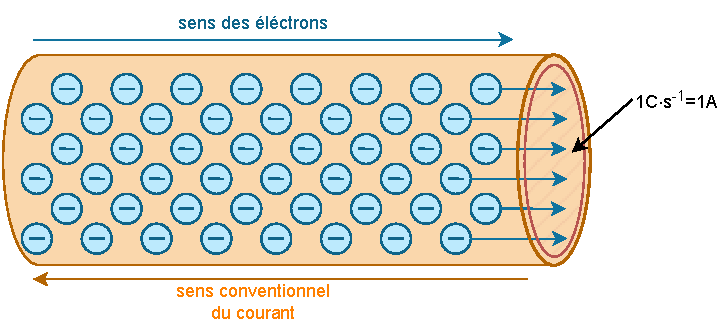
\includegraphics[width=0.7\textwidth]{electron-flow.pdf}
    \caption{Flux de courant dans un conducteur}
\end{figure}
\begin{Todo}
	Aborder la notion de densit\'e de courant. Peut-\^etre dans une section li\'ee \`a l'\'electromagn\'etisme.
	\[
	\vec{j}_S=\int_0^e\vec{j}_S\cdot\vec{dl}
	\]
\end{Todo}

\begin{Note}
\vspace{\baselineskip}
\textbf{Points cl\'es de l’intensit\'e :}
\begin{enumerate}
  \item Elle traduit la vitesse de d\'eplacement des charges dans un conducteur.
  \item Elle est directement li\'ee à la charge et au temps (\(I = Q/t\)).
  \item Elle constitue, avec la tension, la base du calcul de la puissance \'electrique (\(P = U \cdot I\)).
\end{enumerate}
\end{Note}

\subsection{La tension \'electrique}
\begin{Note}
	La notion de courant alternatif sera abord\'ee dans la section (Work In Progress) \Cref{subsec:ac_circuit_theory}.
\end{Note}

La \textbf{tension \'electrique} (ou diff\'erence de potentiel) est la cause
qui met en mouvement les charges \'electriques dans un circuit. Elle
correspond au travail n\'ecessaire pour d\'eplacer une charge \'electrique
unitaire entre deux points. Elle se mesure en \textbf{volts
(\unit{\volt})}.

Math\'ematiquement, la tension est d\'efinie comme :
\[
  U = \frac{W}{Q}
\]
où \(U\) est la tension en volts, \(W\) le travail en joules, et \(Q\) la charge
en coulombs. Ainsi, un volt \'equivaut à un joule par coulomb :
\[
1V=1\frac{J}{C}
\]

% \begin{figure}[!h]
%   \centering
%   \conditionalincludegraphics{src/assets/voltage}{true}{0.5}
%   \caption{Repr\'esentation d’une diff\'erence de potentiel entre deux points}
% \end{figure}

\vspace{\baselineskip}
\begin{Note}
\textbf{Points cl\'es de la tension :}
\begin{enumerate}
  \item Elle est mesur\'ee entre deux points (diff\'erence de potentiel).
  \item Elle constitue la “force motrice” des circuits \'electriques.
  \item Son unit\'e est le volt, \'equivalent à un joule par coulomb.
\end{enumerate}
\end{Note}


\section{Composants de base} \label{subsec:basic_components}
\subsection{R\'esistances} \label{subsec:resistors}
Une r\'esistance est un composant passif qui limite l’intensit\'e du courant
et transforme une partie de l’\'energie \'electrique en chaleur.
Sa relation fondamentale est donn\'ee par la loi d’Ohm :
\[
U = R \cdot I
\]
où \(R\) est exprim\'ee en ohms (\unit{\ohm}).

\begin{figure}[H]
    \centering
    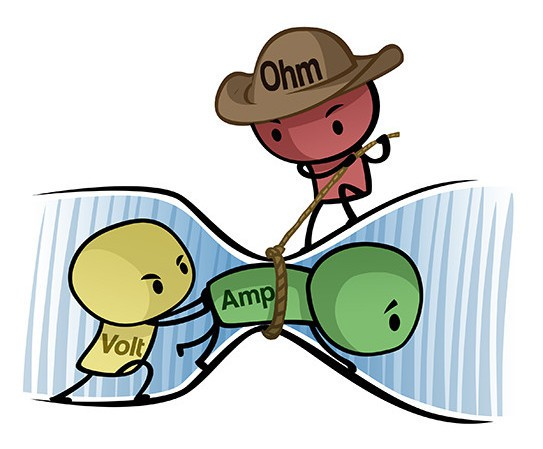
\includegraphics[width=0.6\textwidth]{ohms-law-cartoon}
    \caption{
        \centering
        R\'esistance \'electrique expliqu\'ee par un cowboy. \\\emph{puisque Defred ne veut pas de mes poneys ...}\\
        \textbf{Source~:}
        \href{https://build-electronic-circuits.com/ohms-law}{build-electronic-circuits.com}
    }

\end{figure}


\textbf{Rôle principal :} les r\'esistances servent à fixer des tensions, limiter
le courant dans des composants sensibles (par exemple une LED), ou r\'ealiser
des ponts diviseurs de tension \Cref{fig:voltage-divider}. Elles existent en version fixe (valeur constante)
ou variable (potentiom\`etres, rh\'eostats).

Leur valeur est souvent indiqu\'ee par un code de couleurs :

\begin{table}[H]
\centering
\caption{Code des couleurs pour les r\'esistances (4 bandes)}
\label{tab:resistor_colors}
\begin{tabular}{|l|c|c|c|r|}
\hline
\textbf{Couleur} & \textbf{Chiffre} & \textbf{Multiplicateur} & \textbf{Tol\'erance} & \textbf{Exemple} \\
\hline

\begin{tikzpicture}\fill[black] (0,0) rectangle (0.4,0.4); \end{tikzpicture} Noir & 0 & $10^0$ & - & \si{10\ohm} \\

\begin{tikzpicture}\fill[brown] (0,0) rectangle (0.4,0.4); \end{tikzpicture} Marron & 1 & $10^1$ & ±1\% & \si{10\ohm} \\

\begin{tikzpicture}\fill[red] (0,0) rectangle (0.4,0.4); \end{tikzpicture} Rouge & 2 & $10^2$ & ±2\% & \si{200\ohm} \\

\begin{tikzpicture}\fill[orange] (0,0) rectangle (0.4,0.4); \end{tikzpicture} Orange & 3 & $10^3$ & - & \si{3e3\ohm} \\

\begin{tikzpicture}\fill[yellow] (0,0) rectangle (0.4,0.4); \end{tikzpicture} Jaune & 4 & $10^4$ & - & \si{40e3\ohm} \\

\begin{tikzpicture}\fill[green] (0,0) rectangle (0.4,0.4); \end{tikzpicture} Vert & 5 & $10^5$ & ±0.5\% & \si{500e3\ohm} \\

\begin{tikzpicture}\fill[blue] (0,0) rectangle (0.4,0.4); \end{tikzpicture} Bleu & 6 & $10^6$ & ±0.25\% & \si{1e6\ohm} \\

\begin{tikzpicture}\fill[violet] (0,0) rectangle (0.4,0.4); \end{tikzpicture} Violet & 7 & $10^7$ & ±0.1\% & \si{10e6\ohm} \\

\begin{tikzpicture}\fill[gray] (0,0) rectangle (0.4,0.4); \end{tikzpicture} Gris & 8 & $10^8$ & ±0.05\% & \si{100e6\ohm} \\
\begin{tikzpicture}\fill[white] (0,0) rectangle (0.4,0.4); \draw (0,0) rectangle (0.4,0.4); \end{tikzpicture} Blanc & 9 & $10^9$ & - & \si{1e9\ohm} \\
\begin{tikzpicture}\fill[gold] (0,0) rectangle (0.4,0.4); \end{tikzpicture} Or & - & $10^{-1}$ & ±5\% & \si{0.1\ohm} \\
\begin{tikzpicture}\fill[silver] (0,0) rectangle (0.4,0.4); \end{tikzpicture} Argent & - & $10^{-2}$ & ±10\% & \si{0.01\ohm} \\
\hline
\end{tabular}
\end{table}

\textbf{Association en s\'erie :}
\begin{figure}[H]
    \centering
    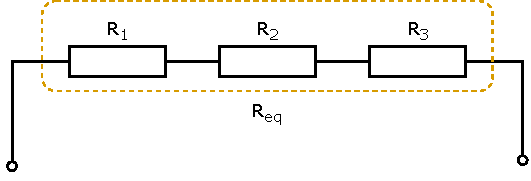
\includegraphics[width=0.8\textwidth]{resistor-series.pdf}
    \caption{\centering
    Association en s\'erie de r\'esistances.\\
    La r\'esistance \'equivalente est la somme des r\'esistances individuelles~:\\
    \(R_{eq} = R_1 + R_2\).}
\end{figure}

\textbf{Association en parall\`ele :}
\begin{figure}[H]
    \fcapside[\FBwidth]{%
        \caption[R\'esistances en parall\`ele.]{
        Association en parall\`ele de r\'esistances.\\
        L’inverse de la r\'esistance \'equivalente est la somme des inverses des r\'esistances individuelles~:
        \vspace{1ex}

        \(\dfrac{1}{R_{eq}} = \dfrac{1}{R_1} + \dfrac{1}{R_2}\).
        }%
        \label{fig:resistor-parallel}%
    }{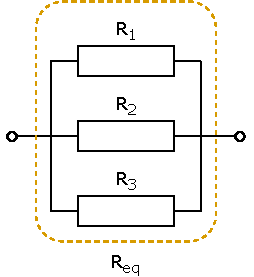
\includegraphics[width=0.4\textwidth]{resistor-parallel.pdf}}%
\end{figure}

\textbf{Pont diviseur de tension :}
\begin{figure}[H]
    \fcapside[\FBwidth]{%
        \caption[Pont diviseur de tension.]{
        Pont diviseur de tension.\\La tension de sortie \(V_{out}\) est une
        fraction de la tension d’entr\'ee \(V_{in}\), d\'etermin\'ee par les valeurs
        des r\'esistances \(R_1\) et \(R_2\)~:\\
        \vspace{\baselineskip}
        \(V_{out} = V_{in}\cdot\dfrac{R_2}{R_1 + R_2}\)
        }%
        \label{fig:voltage-divider}%
    }{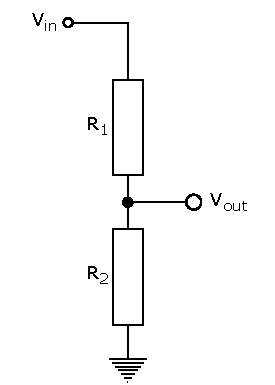
\includegraphics[width=0.4\textwidth]{voltage-divider.pdf}}%
\end{figure}


\textbf{Effet Joule :} lorsqu’un courant traverse une r\'esistance, l’\'energie
\'electrique est dissip\'ee sous forme de chaleur. La puissance thermique d\'egag\'ee
est donn\'ee par :
\[
P = U \cdot I = R \cdot I^2 = \frac{U^2}{R}.
\]
Cet \'echauffement, appel\'e \emph{effet Joule}, peut \^etre utile (ex. : radiateurs,
fils chauffants) ou probl\'ematique (surchauffe des composants, pertes \'energ\'etiques).
Les r\'esistances sont donc conçues avec une puissance nominale (en watts, \unit{\watt})
qu’il ne faut pas d\'epasser pour \'eviter leur destruction.

En pratique, les r\'esistances existent sous diff\'erentes formes :
à couche carbone, à film m\'etallique, bobin\'ees ou int\'egr\'ees dans des circuits imprim\'es.
Leur choix d\'epend à la fois de leur valeur, de leur tol\'erance et de leur puissance maximale.

\subsection{Condensateurs} \label{subsec:capacitors}
Un condensateur stocke de l’\'energie dans un champ \'electrique
entre deux armatures s\'epar\'ees par un isolant (le di\'electrique).
Sa relation fondamentale est :
\[
Q = C \cdot U
\]
où \(C\) est la capacit\'e en farads (\unit{\farad}).
Les condensateurs laissent passer les signaux variables (AC)
et bloquent les signaux constants (DC).
Ils sont utilis\'es pour filtrer les alimentations,
r\'ealiser des circuits r\'esonants, ou encore d\'ecoupler des \'etages \'electroniques.

Les types de condensateurs courants incluent :
\begin{itemize}
  \item \textbf{Condensateurs c\'eramiques :} petit format, faible ESR (r\'esistance \'equivalente en s\'erie), haute fr\'equence.
        Utilis\'es pour d\'ecouplage, filtrage HF et circuits r\'esonants.
  \item \textbf{Condensateurs \'electrolytiques :} grande capacit\'e, polarit\'e à respecter,
        adapt\'es au filtrage d’alimentation et au stockage d’\'energie.
  \item \textbf{Condensateurs à film :} faible perte, non polaris\'es, haute stabilit\'e.
        Applications : circuits audio, filtres, temporisations.
  \item \textbf{Condensateurs tantale :} compacts et stables, polarit\'e à respecter,
        utilis\'es pour alimentation stable et d\'ecouplage.
  \item \textbf{Supercondensateurs / ultracapacitors :} tr\`es grande capacit\'e, d\'echarge rapide,
        pour sauvegarde d’\'energie ou alimentation tampon.
  \item \textbf{Condensateurs à mica :} grande pr\'ecision, faible perte, haute fr\'equence.
        Utilis\'es pour oscillateurs HF et circuits radio.
  \item \textbf{Condensateurs variables :} capacit\'e r\'eglable m\'ecaniquement ou \'electroniquement,
        pour syntonisation\footnote{Glossaire~: \gls{syntonisation}}  d’oscillateurs ou ajustement de filtres.
\end{itemize}
\begin{Note}
	Les notions de filtrage, fr\'equences et imp\'edances seront abord\'ees dans la section (Work In Progress) \Cref{subsec:ac_circuit_theory}.
\end{Note}

\textbf{Association en s\'erie :}
\begin{figure}[H]
    \centering
    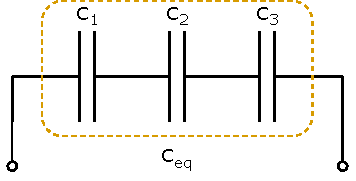
\includegraphics[width=0.6\textwidth]{capacitor-series.pdf}
    \caption{\centering
    Association en s\'erie de condensateurs.\\
    L’inverse de la capacit\'e \'equivalente est la somme des inverses des capacit\'es individuelles
    ~:\\
    \vspace{\baselineskip}
    \(\dfrac{1}{C_{eq}} = \dfrac{1}{C_1} + \dfrac{1}{C_2}\)}
\end{figure}

\textbf{Association en parall\`ele :}
\begin{figure}[H]
    \fcapside[\FBwidth]{%
        \caption[Condensateurs en parall\`ele.]{
        Association en parall\`ele de condensateurs.\\
        La capacit\'e \'equivalente est la somme des capacit\'es individuelles~:\\
        \(C_{eq} = C_1 + C_2\).}%
        \label{fig:capacitor-parallel}%
    }{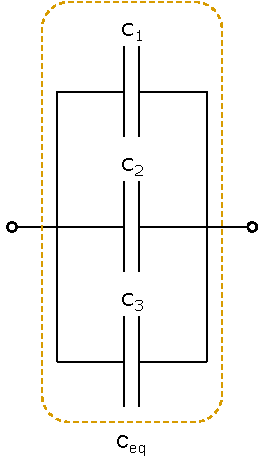
\includegraphics[width=0.4\textwidth]{capacitor-parallel.pdf}}%
\end{figure}

\subsection{Inductances} \label{subsec:inductors}
Une inductance (ou bobine) est un composant passif qui stocke de l’\'energie
dans un champ magn\'etique lorsqu’un courant la traverse.
\[
u(t) = L \frac{di(t)}{dt}
\]
où \(L\) est l’inductance (en henrys, \unit{\henry}) et \(i(t)\) le courant instantan\'e.

\vspace{\baselineskip}
Lorsque le courant est constant (\(\frac{di}{dt} = 0\)), la tension aux bornes
de l’inductance est nulle (\(u = 0\)). Autrement dit, une inductance se comporte
comme un \textbf{court-circuit id\'eal} en r\'egime continu. L’inductance ne s’oppose
donc pas au courant constant, mais uniquement aux variations de courant et \'emet un champ
magn\'etique constant.


\subsection{Diodes} \label{subsec:diodes}
Une diode est un composant semi-conducteur qui laisse passer le courant
dans un sens (polarisation directe) et le bloque dans l’autre (polarisation inverse).
Sa caract\'eristique \(I(V)\) est non lin\'eaire et se rapproche
d’un interrupteur dirig\'e.
\begin{figure}[H]
    \centering
    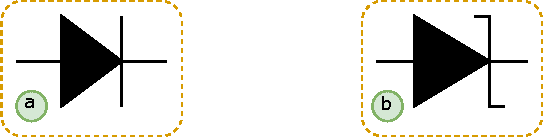
\includegraphics[width=0.5\textwidth]{diodes.pdf}
    \caption{\newline
        \fakecustommacro{a} Symbole d’une diode.\\
        \fakecustommacro{b} Symbole d’une diode Zener.
    }
\end{figure}
Les applications courantes impliquent le redressement dans les alimentations, la protection contre l’inversion de polarit\'e
ou la r\'egulation de tension (diodes Zener).
Certaines diodes sp\'eciales, comme les LED, convertissent l’\'energie \'electrique en lumi\`ere.

\subsection{Transistors} \label{subsec:transistors}
Le transistor est un composant actif central de l’\'electronique moderne.
Il peut amplifier un signal ou agir comme un interrupteur contrôl\'e.
On distingue principalement :
\begin{itemize}
  \item \textbf{BJT (bipolaire)} : le courant de base contrôle
  le courant de collecteur.
  \item \textbf{MOSFET (à effet de champ)} : la tension de grille contrôle
  le courant de drain.
\end{itemize}

\begin{figure}[H]
    \centering
    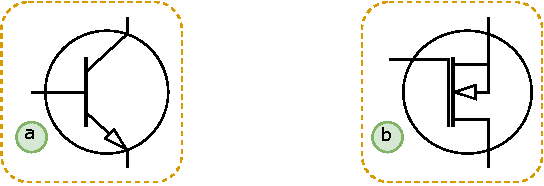
\includegraphics[width=0.6\textwidth]{transistors.pdf}
    \caption{\centering\newline
        \fakecustommacro{a} Symbole d’un transistor NPN (BJT).\\
        \fakecustommacro{b} Symbole d’un transistor N-channel (MOSFET).
    }
\end{figure}

Les transistors sont utilis\'es dans les amplificateurs,
les circuits logiques, les r\'egulateurs, et constituent les briques de base des processeurs.

\section{Lois de Kirchhoff} \label{subsec:kirchhoff}
Les lois de Kirchhoff permettent d’analyser les circuits \'electriques en exprimant
des relations fondamentales entre tensions et courants. Elles sont au nombre de deux :
la loi des nœuds (ou loi des courants) et la loi des mailles (ou loi des tensions).
\subsection{Loi des n{\oe}uds} \label{subsec:noeuds}
\begin{figure}[H]
    \centering
    \fcapside[\FBwidth]{%
        \caption[Loi des n{\oe}uds.]{
            La somme des courants entrants dans un n{\oe}ud est \'egale à la somme des courants sortants ou autrement dit,
            la somme totale des courants est \'egale \`a 0.\\
            Ici~: \(I_1+I_4=I_3+I_2\), ou \(\displaystyle\sum_{i=1}^nI_i=0\)\\
            \vspace{\baselineskip}
            Math\'ematiquement~: \(\displaystyle\sum I_{in} = \displaystyle\sum I_{out}\)
        }%
        \label{fig:kirchhoff-current}%
    }{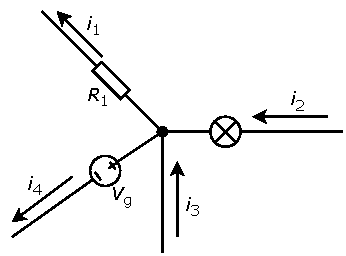
\includegraphics[width=0.4\textwidth]{kirchhoff-current.pdf}}%
\end{figure}

\subsection{Loi des mailles} \label{subsec:mailles}
\begin{figure}[H]
    \centering
    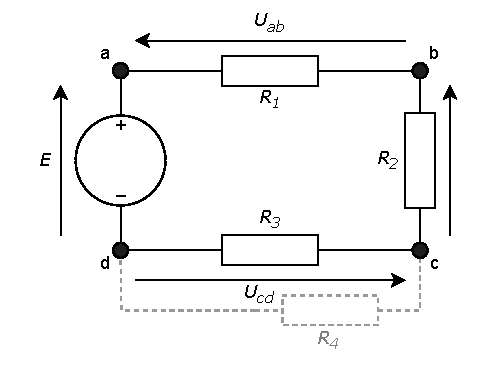
\includegraphics[width=0.6\textwidth]{kirchhoff-voltage.pdf}
    \caption[Loi des mailles.]{
        La somme alg\'ebrique des tensions dans une maille ferm\'ee est nulle.\\
        Ici~: \(E+U_{ab}+U_{bc}+U_{cd}=0\), ou \(\displaystyle\sum_{i=1}^nU_i=0\)\\
        \vspace{\baselineskip}
        Math\'ematiquement~: \(\displaystyle\sum U_{rise} = \displaystyle\sum U_{drop}\)
    }
    \label{fig:kirchhoff-voltage}%
\end{figure}
\begin{Todo}
	Aborder la derivation des lois de Kirchhoff \`a partir des lois de Maxwell.
	\[\sum_i V_i = - \sum_i \int_{\mathcal{P}_i}\mathbf{E}\cdot\mathrm{d}\mathbf{l} = \oint\mathbf{E}\cdot\mathrm{d}\mathbf{l} = 0\]
\end{Todo}

\section{Th\'eor\`emes d'\'equivalence : Th\'evenin et Norton} \label{subsec:thevenin_norton}

Les th\'eor\`emes de Th\'evenin et de Norton permettent de simplifier des circuits
complexes en mod\`eles \'equivalents plus faciles à analyser. Ils sont tr\`es utiles
pour calculer rapidement les tensions et courants vus par une charge.

\subsection{Th\'eor\`eme de Th\'evenin}

Tout circuit lin\'eaire à deux bornes peut \^etre remplac\'e par une source de tension
unique \(E_{th}\) en s\'erie avec une r\'esistance \'equivalente \(R_{th}\).

Prenons un circuit plut\^ot simple\footnote{Tir\'e du cours de Didier Villers},
avec une source de tension et deux r\'esistances, alimentant une charge \(C\) :

\begin{figure}[H]
    \centering
    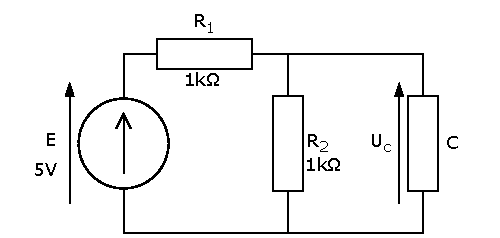
\includegraphics[width=0.6\textwidth]{thevenin/1-Thevenin.pdf}
    \caption{Circuit simple avec une source de tension et deux r\'esistances.}
\end{figure}s
Ici \(E=5V\) et \(R_1=1\unit{\kilo\ohm}\), \(R_2=1\unit{\kilo\ohm}\).\\

On commence d'abord par ouvrir le circuit pour mesurer la tension à vide \(E_{th}\) :
\begin{figure}[H]
    \centering
    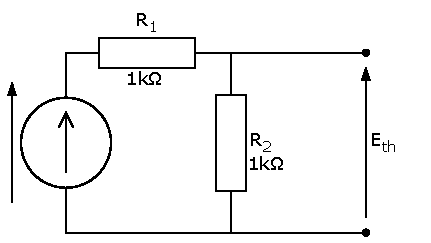
\includegraphics[width=0.6\textwidth]{thevenin/2-Thevenin.pdf}
    \caption{Ouverture du circuit pour mesurer la tension à vide \(E_{th}\).}
\end{figure}
\(E_{th}\) se calcule facilement avec le pont diviseur de tension :
\[
E_{th} = E \cdot \frac{R_2}{R_1+R_2} = 5\unit{\volt} \cdot \frac{1\unit{\kilo\ohm}}{1\unit{\kilo\ohm}+1\unit{\kilo\ohm}} = 2.5\unit{\volt}
\]

Ensuite, on remplace la source de tension par un court-circuit et on calcule la
r\'esistance \'equivalente \(R_{th}\) vue des bornes de la charge \(C\) :
\begin{figure}[H]
    \centering
    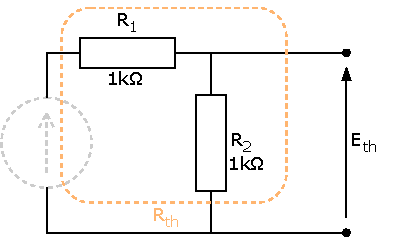
\includegraphics[width=0.6\textwidth]{thevenin/2-5Thevenin.pdf}
    \caption{Remplacement de la source de tension par un court-circuit pour calculer \(R_{th}\).}
\end{figure}
\(R_{th}\) se calcule facilement avec la formule des r\'esistances en parall\`ele :
\[
R_{th} = \frac{R_1 \cdot R_2}{R_1 + R_2} = \frac{1\unit{\kilo\ohm} \cdot 1\unit{\kilo\ohm}}{1\unit{\kilo\ohm} + 1\unit{\kilo\ohm}} = 500\unit{\ohm}
\]
On peut maintenant dessiner le circuit \'equivalent de Th\'evenin :
\begin{figure}[H]
    \centering
    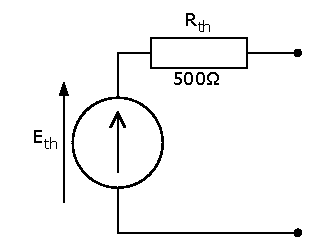
\includegraphics[width=0.6\textwidth]{thevenin/3-Thevenin.pdf}
    \caption{Circuit \'equivalent de Th\'evenin.}
    \label{fig:thevenin-equivalent}
\end{figure}
En prenant \(R_c=500\unit{\ohm}\).\\
On peut facilement calculer la tension \(U_{c}\) aux bornes de la charge \(C\) avec le pont diviseur de tension :
\[
U_{c} = E_{th} \cdot \frac{R_c}{R_{th} + R_c} = 2.5\unit{\volt} \cdot \frac{500\unit{\ohm}}{500\unit{\ohm} + 500\unit{\ohm}} = 1.25\unit{\volt}
\]

\begin{figure}[H]
    \centering
    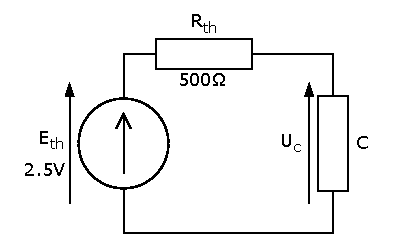
\includegraphics[width=0.6\textwidth]{thevenin/4-Thevenin.pdf}
    \caption{Calcul de la tension \(U_{c}\) aux bornes de la charge \(C\).}
\end{figure}



\subsection{Th\'eor\`eme de Norton}

Tout circuit lin\'eaire à deux bornes peut \^etre remplac\'e par une source de courant
unique \(I_{n}\) en parall\`ele avec une r\'esistance \'equivalente \(R_{n}\). Il permet
de simplifier l’analyse des circuits en remplaçant des r\'eseaux complexes de r\'esistances
invariantes dans le temps par une source de courant et une r\'esistance \'equivalente.

Prenons un circuit plut\^ot simple\footnote{Tir\'e du cours de Didier Villers}, avec une source de courant et deux r\'esistances
en s\'erie, alimentant une charge \(C\) :
\begin{figure}[H]
    \centering
    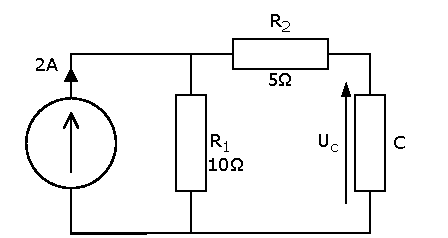
\includegraphics[width=0.6\textwidth]{norton/1-Norton.pdf}
    \caption{Circuit simple avec une source de courant et deux r\'esistances en s\'erie.}
\end{figure}

On commence d'abord par court-circuiter la charge \(C\) pour mesurer le courant de court-circuit \(I_{n}\) :
\begin{figure}[H]
    \centering
    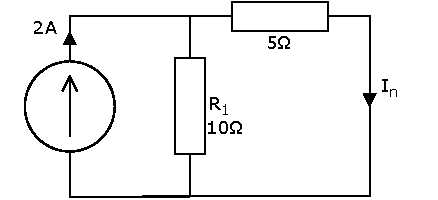
\includegraphics[width=0.6\textwidth]{norton/2-Norton.pdf}
    \caption{Court-circuit de la charge \(C\) pour mesurer le courant de court-circuit \(I_{n}\).}
\end{figure}

\(I_{n}\) se calcule facilement avec le pont diviseur de courant :
\[
I_{n} = I \cdot \frac{R_1}{R_1 + R_2} = 2\unit{\ampere} \cdot \frac{10\unit{\ohm}}{10\unit{\ohm} + 5\unit{\ohm}} = 1.33\unit{\ampere}
\]

Ensuite, on remplace la source de courant par un circuit ouvert et on calcule la
r\'esistance \'equivalente \(R_{n}\) vue des bornes de la charge \(C\) :
\begin{figure}[H]
    \centering
    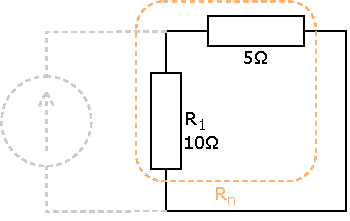
\includegraphics[width=0.6\textwidth]{norton/2-5Norton.pdf}
    \caption{Remplacement de la source de courant par un circuit ouvert pour calculer \(R_{n}\).}
\end{figure}

\(R_{n}\) se calcule facilement avec la formule des r\'esistances en s\'erie :
\[
R_{n} = R_{1} + R_{2} = 10\unit{\ohm} + 5\unit{\ohm} = 15\unit{\ohm}
\]

On peut maintenant dessiner le circuit \'equivalent de Norton :
\begin{figure}[H]
    \centering
    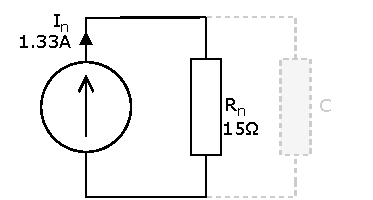
\includegraphics[width=0.6\textwidth]{norton/3-Norton.pdf}
    \caption{Circuit \'equivalent de Norton.}
    \label{fig:norton-equivalent}
\end{figure}
En prenant \(R_c=500\unit{\ohm}\).\\
On peut facilement calculer la tension \(U_{c}\) aux bornes de la charge \(C\) avec le pont diviseur de tension :
\[
U_{c} = I_{n} \cdot \frac{R_{n} \cdot R_{c}}{R_{n} + R_{c}} = 1.33\unit{\ampere} \cdot \frac{15\unit{\ohm} \cdot 500\unit{\ohm}}{15\unit{\ohm} + 500\unit{\ohm}} = 19.37\unit{\volt}
\]

\begin{figure}[H]
	\centering
    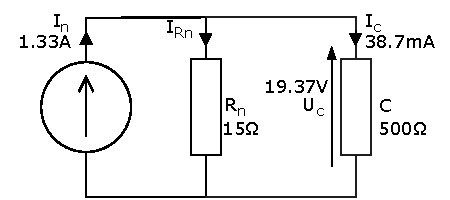
\includegraphics[width=0.6\textwidth]{norton/4-Norton.pdf}
    \caption{Calcul de la tension \(U_{c}\) aux bornes de la charge \(C\).}
\end{figure}

\subsection{Relation entre Th\'evenin et Norton}

Il est souvent pratique de passer d'une repr\'esentation de Th\'evenin à une
repr\'esentation de Norton, et vice-versa, les deux repr\'esentations sont
strictement \'equivalentes. Voici les relations entre les param\`etres des deux
mod\`eles :
\begin{align*}
  E_{th} & = I_{n} \cdot R_{n} \\
  I_{n} & = \frac{E_{th}}{R_{th}} \\
  R_{th} & = R_{n}
\end{align*}

\begin{Note}
	Points cl\'es des th\'eor\`emes de Th\'evenin et Norton :
    \begin{enumerate}
        \item Ils permettent de simplifier des circuits complexes en mod\`eles \'equivalents plus simples.
        \item Le th\'eor\`eme de Th\'evenin utilise une source de tension en s\'erie avec une r\'esistance.
        \item Le th\'eor\`eme de Norton utilise une source de courant en parall\`ele avec une r\'esistance.
        \item Les deux mod\`eles sont \'equivalents et peuvent \^etre convertis l’un en l’autre.
    \end{enumerate}
\end{Note}

\section{Theor\`eme de Millman} \label{subsec:millman}
Le th\'eor\`eme de Millman est une m\'ethode efficace pour analyser des circuits \'electriques comportant plusieurs branches en parall\`ele aliment\'ees par des sources de tension et de courant. Il permet de calculer rapidement la tension commune aux nœuds d’un circuit complexe.
